\section{Introduction}\label{intro}

Optimization problems are problems in which the goal is to locate a set of inputs $x \in \mathbf{R}^{n}$ that result in the minima or maxima of a target objective function. In this thesis the problem of minimizing an objective function often called a cost/loss function will be considered. Such an optimization problem takes the form:
\begin{equation*}\label{eq:1}\tag{1.1}
\begin{aligned}
    &\text{minimize} \ f_{0}(x) \\
    &\text{subject to} \ f_{i}(x) \leq b_{i}, \text{  } i=1,\ldots,m 
\end{aligned}
\end{equation*}
Here the vector $x=(x_{1},\ldots,x_{n})$ is called the optimization variable, the function $f_{0}: \mathbf{R}^{n} \longrightarrow \mathbf{R}$ is the objective function, the functions $f_{i}: \mathbf{R}^{n} \longrightarrow \mathbf{R}, \text{  }i=1,\ldots,m$ are the constraint functions and the constants $b_{1},\ldots,b_{m}$ are the bounds for the constraints. A vector $x^{*}$ is called an optimal solution to the problem if the function $f_{0}$ attains either a local or a global minimum at $x^{*}$. 

In the fields of machine learning and deep learning, optimization is used to train models that can perform a desired task. In machine learning, the objective function $f_0$ represents a loss function that measures the discrepancy between the model's predictions and the true target values. The optimization problem is then to find the parameters of the model that minimize this loss function, subject to any constraints specified by the constraint functions $f_i$ and bounds $b_i$. In deep learning, the model is typically a neural network, with the optimization variable $x$ representing the weights and biases of the network. The optimization problem is then to find the values of the weights and biases that result in the best performance on a given task, as measured by the loss function. The importance of optimization in machine learning and deep learning lies in its ability to train models that can generalize well to new data and perform well on the desired task. The optimization problem provides a framework for finding the best possible parameters of the model, given the loss function and any constraints, and is a crucial step in the training process for machine learning and deep learning models.     

We generally consider different classes of optimization problems that differ in the form of the objective function and of its constraints. For example, the optimization problem \ref{eq:1} is said to be a linear problem if the objective function $f_{0}$ and constraints $f_{1},\ldots,f_{m}$ are linear. Then these functions satisfy:
\begin{equation*}\label{eq:2}\tag{1.2}
\begin{aligned}
    &f_{i}(\alpha x + \beta y) = \alpha f_{i}(x) + \beta f_{i}(y) \text{ } \text{,}\text{     }\text{  }i=0,\ldots,m
\end{aligned}
\end{equation*}
For all $x,y \in \mathbf{R}^{n}$ and all $\alpha,\beta \in \mathbf{R}$. An optimization problem that is not linear is called non-linear. One particular class of optimization problems called convex optimization problems has proven to be very useful. A convex optimization problem is a problem in which the objective function $f_{0}$ and the constraints $f_{1},\ldots,f_{m}$ are convex, which means they satisfy the inequality:
\begin{equation*}\label{eq:3}\tag{1.3}
\begin{aligned}
    &f_{i}(\alpha x + \beta y) \leq \alpha f_{i}(x) + \beta f_{i}(y) \text{ } \text{,}\text{    }\text{  }i=0,\ldots,m
\end{aligned}
\end{equation*}
For all $x,y \in \mathbf{R}^{n}$ and all $\alpha,\beta \in \mathbf{R}$ with $\alpha + \beta = 1$ and $\alpha \geq 0$, $\beta \geq 0$. Convexity is more general than linearity. In the situation of convex optimization the equality in \ref{eq:2} is replaced by an inequality in \ref{eq:3} which only holds for certain values of $\alpha$ and $\beta$. Convex optimization can be considered to be a generalization of linear optimization. The main important property of convex functions is that they have a single minimum which is also the global minimum. This property makes convex optimization well-suited for problems where there is a clear and unique optimal solution. 
\begin{comment}
Convex optimization is useful in machine learning and deep learning, since many common loss functions are convex, making it possible to use convex optimization to find the best parameters for the model. 
\end{comment}
Convex optimization problems can often be solved efficiently using well-established optimization algorithms, such as gradient descent. These algorithms can converge relatively quickly to a global minimum, but the convergence rate can depend on various factors, such as the dimensionality of the problem. For convex loss functions, convex optimization provides a guarantee of finding the global minimum of the loss function. A simple example of a convex objective function on $\mathbf{R}^2$ would be the following: 
\begin{equation*}\label{eq:10}\tag{1.4}
\begin{aligned}
    &f(x) = \frac{1}{2}(x_{1}^{2} + 10x_{2}^{2})
\end{aligned}
\end{equation*}
This function is a quadratic function that describes an elliptical bowl and its graph has a parabolic shape.
Clearly the optimal solution is $x^{*} = (0,0)$ with $f(x^{*}) = 0$.\newpage An example of a non-convex function on $\mathbf{R}^2$ is the following: 
\begin{equation*}\label{eq:11}\tag{1.5}
\begin{aligned}
    &g(x) = \frac{\sin\left(0.5x_1^2 - 0.25x_2^2 + 3\right)}{0.5 + 0.25x_1^2 + x_2^2}
\end{aligned}
\end{equation*}
By visual inspection of the graph of this function, one can easily see that $g$ is not convex, since it has many local minima and maxima. The convex function $f$ and non-convex function $g$ can be visualized using computational tools\footnote{See line~\ref{line:p1} to~\ref{line:p2} for the code}. The illustration of these functions is presented in the figures below.

\begin{figure}[h]
  \centering
  \begin{minipage}[b]{0.42\textwidth}
    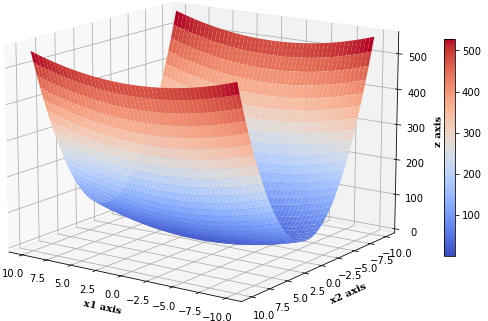
\includegraphics[width=\textwidth]{Pictures/3D plot of ellipsoid.png}
    \caption{3D plot of $f$}\label{fig:ellipsoid_3D}
  \end{minipage}
  \hspace{0.3cm} 
  \begin{minipage}[b]{0.42\textwidth}
    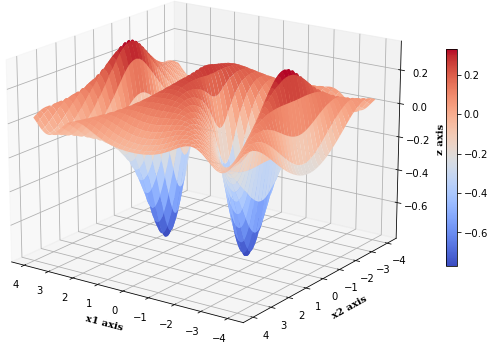
\includegraphics[width=\textwidth]{Pictures/3D plot of non convex.png}
    \caption{3D plot of $g$}\label{fig:Nonconvex_3D}
  \end{minipage}
\end{figure}
    
























------